\documentclass[10pt]{article}
\usepackage[margin=0.65in]{geometry}
\usepackage{graphicx,hyperref,booktabs}
\hypersetup{colorlinks=true,urlcolor=blue}
\setlength{\parindent}{0pt}
\setlength{\parskip}{5pt}
\begin{document}
\begin{center}\Large Native hashed ECDLP through ECBench\\
\normalsize Engineering and pre-data feasibility protocol -- 2026-10-30\end{center}

The implemented native library now has source, selector, exact-width and
partial-relation arms. The development suites pass 90 tests in crypto and
96 in cryptanalysis; the observer/default-policy control preserves the full
certificate, RNG state and metered work. The native end-to-end control checks
scalars independently and replays both successful and exhausted records.
No scientific session or runtime result is reported here.

\begin{center}
\begin{tabular}{rrrr}
\toprule Field bits & Subgroup $r$ & Targets & Measured rounds\\\midrule
10 & 823 & 8 & 5\\12 & 3889 & 8 & 5\\14 & 16231 & 8 & 5\\16 & 65003 & 8 & 5\\\bottomrule
\end{tabular}
\end{center}
All four curves have registered ICV1 and readable EC1 identifiers in
\texttt{plan.txt}. Nine arms, one warmup and five measured rounds give
1,728 planned executions (1,440 measured). All native arms use the same explicit
five-million-step, $m=2$, $\tau=32$ and resource policies. Rho, rho A/A, a newer
rho positive control, selector A/A and a bundled IC comparator are retained.

\begin{center}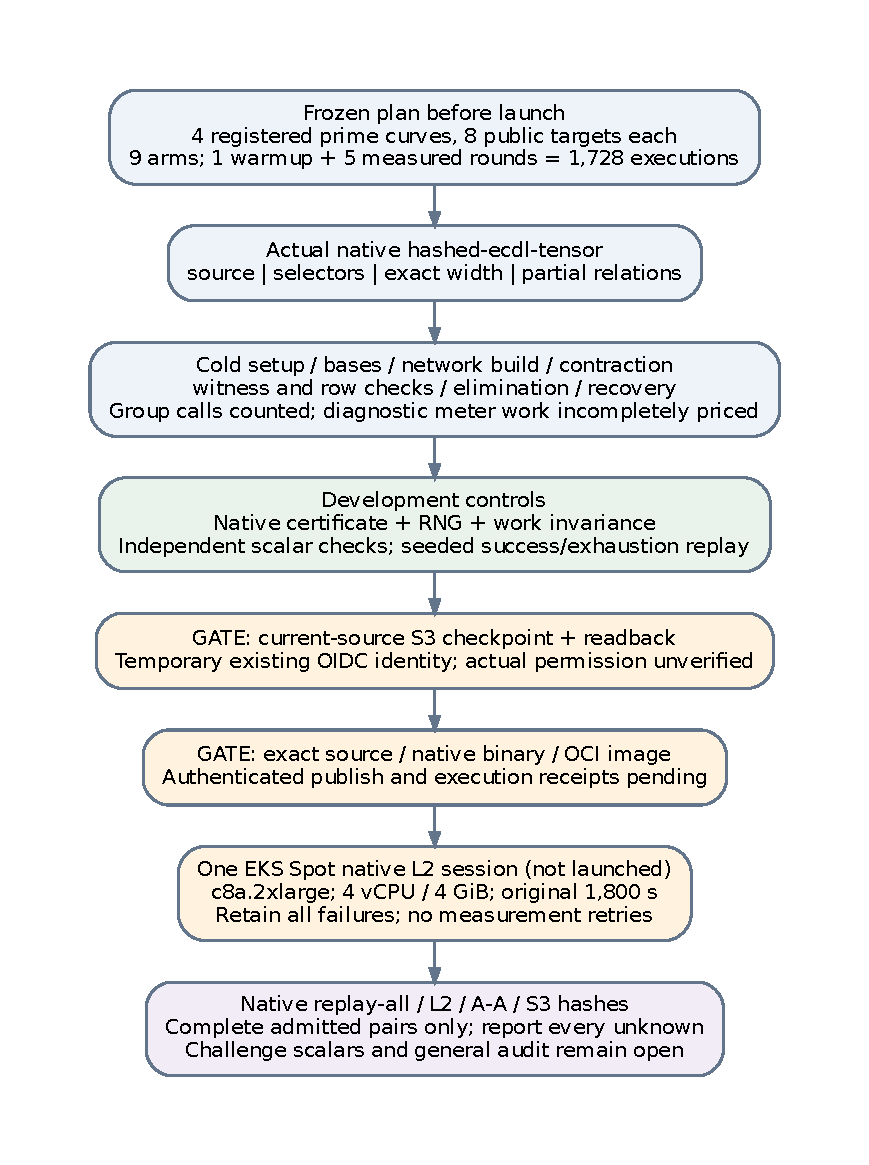
\includegraphics[height=4.45in]{pipeline.pdf}\end{center}

\textbf{Scope.} Every native group call is counted; other arithmetic is not
fully inventoried or priced. Native $S$ is a lower bound, and clocks include
observation overhead. A budget exhaustion is unknown, never a fast success;
incomplete arms prevent complete comparisons. The 1,800-second original job
budget is a hard ceiling, not a measured runtime prediction. No matched native
preflight, power, scaling or fastest-tool claim is made. The first warmups are
recorded without changing the frozen plan. The original 60/24 A/B study,
profiling, binary/full schoolbook pipelines, both challenge scalars and the
independent general audit remain open.

\textbf{Evidence and sources.} See \texttt{README.md}, \texttt{protocol.json},
\texttt{spec.json} and the lossless logs/source manifests in
\texttt{implementation/}. Two malformed upstream test modules were restored
byte-for-byte from their original merge parents without removing assertions.
The diagram describes planned execution and pending gates, since there are
no scientific measurements to plot. The source is the pinned
\href{https://github.com/bochum-crypto/subexponential-ecdl/tree/1ee44e562b1b9a50ea339f3b8f81112b5a24b96f}{Bochum reduction},
the repository's finite-backend implementation, ECBench unit/replay rules and
Iso Lab access/harness contracts. No theorem or source packet guard changes.
\end{document}
